%! Author = paulsen
%! Date = 25.11.23

\begin{frame}{KDE Plasma}
    \section{KDE Plasma}\label{sec:KDE-Plasma}
\end{frame}

\begin{frame}{Einstellungen}
    \subsection{Plasma Einstellungen}\label{subsec:plasma-einstellungen}
    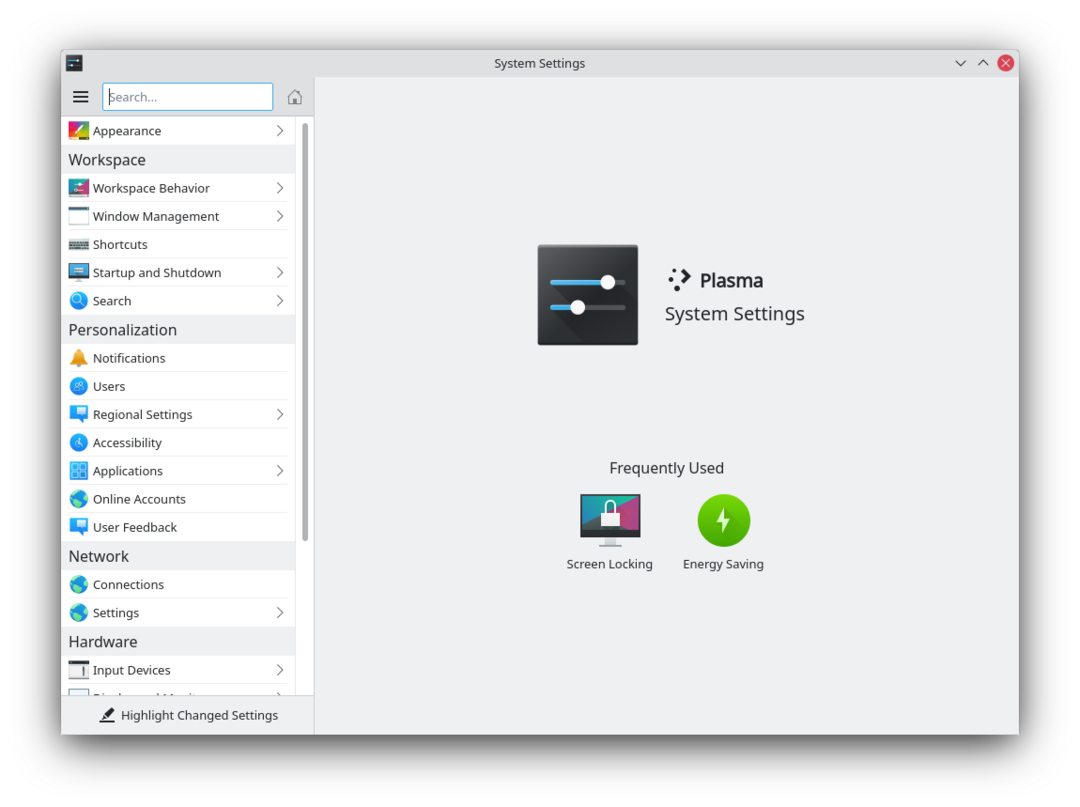
\includegraphics[width=11cm]{plasma-systemsettings}
\end{frame}

\begin{frame}{Einstellungen}

    \vspace{0.5cm}
    \begin{alertblock}{Aufgabe}
        Klicke dich durch die Einstellungen und erledige diese Aufgaben:

        \pause
        \begin{itemize}
            \item Ändere das Hintergrundbild\pause
            \item Ändere dein Nutzerpasswort\pause
            \item Verändere die systemweite Akzentfarbe\pause
            \item Erstelle mehrere Virtuelle Desktops\pause
            \item Verändere die Shortcuts zum Wechseln der Desktops
        \end{itemize}
    \end{alertblock}
\end{frame}

\begin{frame}{Widgets}
    \subsection{Widgets}\label{subsec:widgets}
    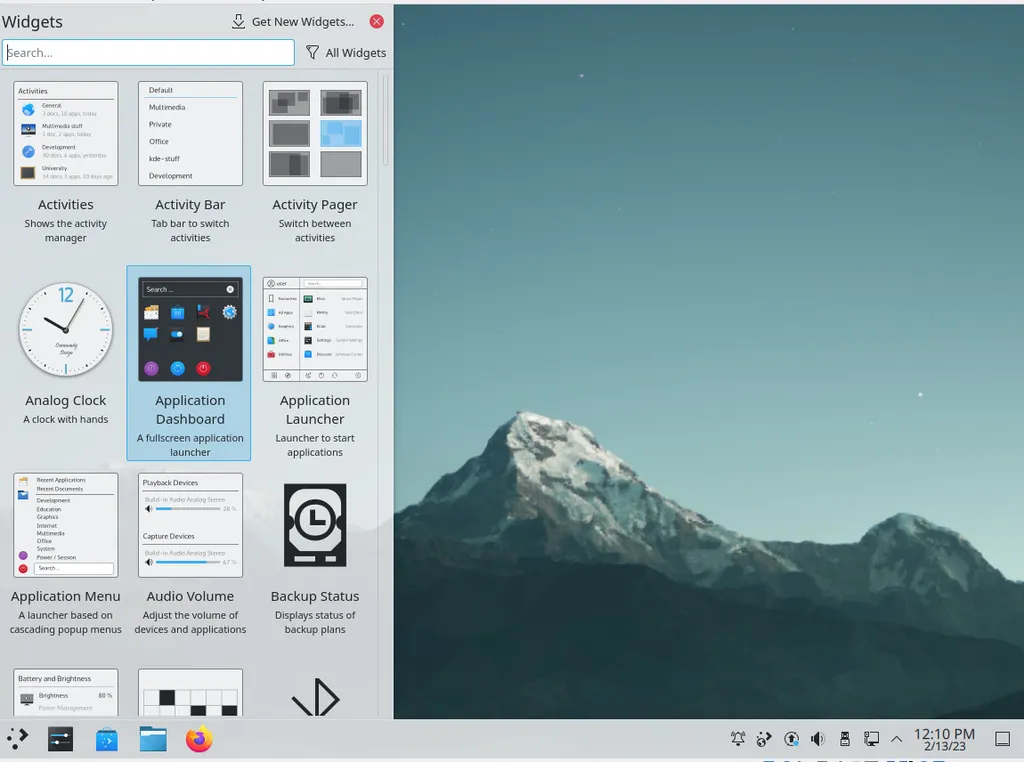
\includegraphics[width=11cm]{plasma-widgets}
\end{frame}

\begin{frame}{Widgets}

    Widgets sind kleine visuelle Anwendungen, die zur Anzeige von Informationen oder Shortcuts
    dienen.

    \pause

    \begin{itemize}
        \item Vor dem Desktophintergrund anzeigbar\pause
        \item Kann in die Desktop-Leiste eingefügt werden\pause
        \item Benutzer-Widgets können nachinstalliert werden
    \end{itemize}

    \pause
    \vspace{0.5cm}
    \begin{alertblock}{Aufgabe}
        \begin{itemize}
            \item Füge ein Mediaplayer-Widget in das Desktop-Panel ein.
            \item Verschiebe das Desktop-Panel an einen anderen Bildschirmrand und passe die Größe der Leiste an.
        \end{itemize}
    \end{alertblock}
\end{frame}

\begin{frame}{Vaults}
    \subsection{Vaults}\label{subsec:vaults}
    \begin{itemize}
        \item Verschlüsselte Ordner\pause
        \item Icon versteckt in Benachrichtigungsleiste\pause
        \item Ordner können mit der Cloud oder anderen Speichermedien synchronisiert und
        transportiert werden
    \end{itemize}

    \pause
    \vspace{0.5cm}
    \begin{alertblock}{Aufgabe}
        Erstelle einen mit Passwort verschlüsselten Ordner
    \end{alertblock}
\end{frame}